\documentclass{standalone}
\usepackage{tikz, xcolor}
\usetikzlibrary{shapes,arrows}

\begin{document}

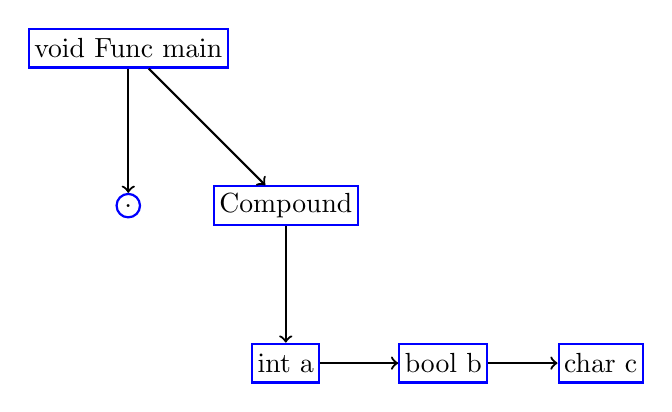
\begin{tikzpicture}[thick, scale=2.0]
\tikzstyle{vertexr}=[rectangle, draw=blue, thick, minimum size=14pt, inner sep=2pt]
\tikzstyle{vertexc}=[circle, draw=blue, thick, inner sep=2pt]
\tikzstyle{drawstyle}=[thick, ->]

\node[vertexr] (G0x0) at (0,0) {void Func main};
\node[vertexc] (G0x1) at (0,-1) {.};
\draw[drawstyle] (G0x0) -- (G0x1);
\node[vertexr] (G1x1) at (1,-1) {Compound};
\node[vertexr] (G1x2) at (1,-2) {int a};
\node[vertexr] (G2x2) at (2,-2) {bool b};
\node[vertexr] (G3x2) at (3,-2) {char c};
\draw[drawstyle] (G2x2) -- (G3x2);
\draw[drawstyle] (G1x2) -- (G2x2);
\draw[drawstyle] (G1x1) -- (G1x2);
\draw[drawstyle] (G0x0) -- (G1x1);
\end{tikzpicture}
\end{document}
Number of warnings: 0
Number of errors: 0
